% Options for packages loaded elsewhere
\PassOptionsToPackage{unicode}{hyperref}
\PassOptionsToPackage{hyphens}{url}
%
\documentclass[
]{book}
\usepackage{amsmath,amssymb}
\usepackage{iftex}
\ifPDFTeX
  \usepackage[T1]{fontenc}
  \usepackage[utf8]{inputenc}
  \usepackage{textcomp} % provide euro and other symbols
\else % if luatex or xetex
  \usepackage{unicode-math} % this also loads fontspec
  \defaultfontfeatures{Scale=MatchLowercase}
  \defaultfontfeatures[\rmfamily]{Ligatures=TeX,Scale=1}
\fi
\usepackage{lmodern}
\ifPDFTeX\else
  % xetex/luatex font selection
\fi
% Use upquote if available, for straight quotes in verbatim environments
\IfFileExists{upquote.sty}{\usepackage{upquote}}{}
\IfFileExists{microtype.sty}{% use microtype if available
  \usepackage[]{microtype}
  \UseMicrotypeSet[protrusion]{basicmath} % disable protrusion for tt fonts
}{}
\makeatletter
\@ifundefined{KOMAClassName}{% if non-KOMA class
  \IfFileExists{parskip.sty}{%
    \usepackage{parskip}
  }{% else
    \setlength{\parindent}{0pt}
    \setlength{\parskip}{6pt plus 2pt minus 1pt}}
}{% if KOMA class
  \KOMAoptions{parskip=half}}
\makeatother
\usepackage{xcolor}
\usepackage{color}
\usepackage{fancyvrb}
\newcommand{\VerbBar}{|}
\newcommand{\VERB}{\Verb[commandchars=\\\{\}]}
\DefineVerbatimEnvironment{Highlighting}{Verbatim}{commandchars=\\\{\}}
% Add ',fontsize=\small' for more characters per line
\usepackage{framed}
\definecolor{shadecolor}{RGB}{248,248,248}
\newenvironment{Shaded}{\begin{snugshade}}{\end{snugshade}}
\newcommand{\AlertTok}[1]{\textcolor[rgb]{0.94,0.16,0.16}{#1}}
\newcommand{\AnnotationTok}[1]{\textcolor[rgb]{0.56,0.35,0.01}{\textbf{\textit{#1}}}}
\newcommand{\AttributeTok}[1]{\textcolor[rgb]{0.13,0.29,0.53}{#1}}
\newcommand{\BaseNTok}[1]{\textcolor[rgb]{0.00,0.00,0.81}{#1}}
\newcommand{\BuiltInTok}[1]{#1}
\newcommand{\CharTok}[1]{\textcolor[rgb]{0.31,0.60,0.02}{#1}}
\newcommand{\CommentTok}[1]{\textcolor[rgb]{0.56,0.35,0.01}{\textit{#1}}}
\newcommand{\CommentVarTok}[1]{\textcolor[rgb]{0.56,0.35,0.01}{\textbf{\textit{#1}}}}
\newcommand{\ConstantTok}[1]{\textcolor[rgb]{0.56,0.35,0.01}{#1}}
\newcommand{\ControlFlowTok}[1]{\textcolor[rgb]{0.13,0.29,0.53}{\textbf{#1}}}
\newcommand{\DataTypeTok}[1]{\textcolor[rgb]{0.13,0.29,0.53}{#1}}
\newcommand{\DecValTok}[1]{\textcolor[rgb]{0.00,0.00,0.81}{#1}}
\newcommand{\DocumentationTok}[1]{\textcolor[rgb]{0.56,0.35,0.01}{\textbf{\textit{#1}}}}
\newcommand{\ErrorTok}[1]{\textcolor[rgb]{0.64,0.00,0.00}{\textbf{#1}}}
\newcommand{\ExtensionTok}[1]{#1}
\newcommand{\FloatTok}[1]{\textcolor[rgb]{0.00,0.00,0.81}{#1}}
\newcommand{\FunctionTok}[1]{\textcolor[rgb]{0.13,0.29,0.53}{\textbf{#1}}}
\newcommand{\ImportTok}[1]{#1}
\newcommand{\InformationTok}[1]{\textcolor[rgb]{0.56,0.35,0.01}{\textbf{\textit{#1}}}}
\newcommand{\KeywordTok}[1]{\textcolor[rgb]{0.13,0.29,0.53}{\textbf{#1}}}
\newcommand{\NormalTok}[1]{#1}
\newcommand{\OperatorTok}[1]{\textcolor[rgb]{0.81,0.36,0.00}{\textbf{#1}}}
\newcommand{\OtherTok}[1]{\textcolor[rgb]{0.56,0.35,0.01}{#1}}
\newcommand{\PreprocessorTok}[1]{\textcolor[rgb]{0.56,0.35,0.01}{\textit{#1}}}
\newcommand{\RegionMarkerTok}[1]{#1}
\newcommand{\SpecialCharTok}[1]{\textcolor[rgb]{0.81,0.36,0.00}{\textbf{#1}}}
\newcommand{\SpecialStringTok}[1]{\textcolor[rgb]{0.31,0.60,0.02}{#1}}
\newcommand{\StringTok}[1]{\textcolor[rgb]{0.31,0.60,0.02}{#1}}
\newcommand{\VariableTok}[1]{\textcolor[rgb]{0.00,0.00,0.00}{#1}}
\newcommand{\VerbatimStringTok}[1]{\textcolor[rgb]{0.31,0.60,0.02}{#1}}
\newcommand{\WarningTok}[1]{\textcolor[rgb]{0.56,0.35,0.01}{\textbf{\textit{#1}}}}
\usepackage{longtable,booktabs,array}
\usepackage{calc} % for calculating minipage widths
% Correct order of tables after \paragraph or \subparagraph
\usepackage{etoolbox}
\makeatletter
\patchcmd\longtable{\par}{\if@noskipsec\mbox{}\fi\par}{}{}
\makeatother
% Allow footnotes in longtable head/foot
\IfFileExists{footnotehyper.sty}{\usepackage{footnotehyper}}{\usepackage{footnote}}
\makesavenoteenv{longtable}
\usepackage{graphicx}
\makeatletter
\def\maxwidth{\ifdim\Gin@nat@width>\linewidth\linewidth\else\Gin@nat@width\fi}
\def\maxheight{\ifdim\Gin@nat@height>\textheight\textheight\else\Gin@nat@height\fi}
\makeatother
% Scale images if necessary, so that they will not overflow the page
% margins by default, and it is still possible to overwrite the defaults
% using explicit options in \includegraphics[width, height, ...]{}
\setkeys{Gin}{width=\maxwidth,height=\maxheight,keepaspectratio}
% Set default figure placement to htbp
\makeatletter
\def\fps@figure{htbp}
\makeatother
\setlength{\emergencystretch}{3em} % prevent overfull lines
\providecommand{\tightlist}{%
  \setlength{\itemsep}{0pt}\setlength{\parskip}{0pt}}
\setcounter{secnumdepth}{5}
\usepackage{booktabs}
\ifLuaTeX
  \usepackage{selnolig}  % disable illegal ligatures
\fi
\usepackage[]{natbib}
\bibliographystyle{plainnat}
\usepackage{bookmark}
\IfFileExists{xurl.sty}{\usepackage{xurl}}{} % add URL line breaks if available
\urlstyle{same}
\hypersetup{
  pdftitle={Relatório Velocidades},
  pdfauthor={Arthur Hideio Noguti},
  hidelinks,
  pdfcreator={LaTeX via pandoc}}

\title{Relatório Velocidades}
\author{Arthur Hideio Noguti}
\date{2024-07-26}

\begin{document}
\maketitle

{
\setcounter{tocdepth}{1}
\tableofcontents
}
\chapter{Introdução}\label{intro}

Esse documento possui a finalidade de transmitir meus pensamentos sobre o que foi feito em R no relatório de velocidades e também serve como uma forma de treinamento para minhas habilidades em \emph{markdown}

\section{Partes}\label{partes}

Esse documento está dividido em 5 partes, sendo elas:

\begin{itemize}
\tightlist
\item
  Indicadores radares/frota;\\
\item
  Indicador radares/Km;\\
\item
  Indicador mortalidade;\\
\item
  Quantidade de radares por limite de velocidde;\\
\item
  Correlações entre indicadores.
\end{itemize}

\section{Observações}\label{observauxe7uxf5es}

Algumas bases de dados serão importadas pelo \href{https://github.com/ONSV}{\emph{GitHub} do ONSV}, entretando a base de dados que representa a quantidade de radares com suas características e da extensão das rodovias em cada unidade da federação serão importadas diretamente do computador, para a utilização dessas, você deverá baixar o arquivo excel e mudar o diretório do script quando tiver alguma função do tipo \texttt{read\_csv(SEU\ DIRETÓRIO)}

\chapter{Indicadores radares/frota}\label{radar-frota}

\section{Bibliotecas}\label{bibliotecas}

Para realizar o cálculo dos indicadores foram utilizados as seguintes bibliotecas:

\begin{Shaded}
\begin{Highlighting}[]
\FunctionTok{library}\NormalTok{(tidyverse)}
\FunctionTok{library}\NormalTok{(readxl)}
\CommentTok{\# devtools::install\_github("jotasaraiva/fleetbr")}
\FunctionTok{library}\NormalTok{(fleetbr)}
\end{Highlighting}
\end{Shaded}

Note que tem uma parte do \emph{script} que está depois de um \texttt{\#}, caso vocẽ não tenha instalado em sua máquina a base de dados sobre a frota de veículos no Brasil basta retirar o \texttt{\#} e rodar o \emph{script}. Eu não vou entrar em detalhes técnicos nesse documento, como por exemplo o que significa cada indicador e sua função, pois isto é apresentado no relatório em si.

\section{Pré processamento}\label{pruxe9-processamento}

Além dessa base de dados, será necessário também a base sobre os radares, que será importado pelo arquivo .csv, como é demonstrado pelo \emph{script} abaixo:

\begin{Shaded}
\begin{Highlighting}[]
\NormalTok{radares }\OtherTok{\textless{}{-}} \FunctionTok{read\_xlsx}\NormalTok{(}\StringTok{"/home/silvana/Downloads/INDICADORES\_RADARES\_VELOCIDADE\_UF (indicador velocidade, infrações, mortalidade)).xlsx"}\NormalTok{, }\AttributeTok{sheet =} \DecValTok{2}\NormalTok{)}
\end{Highlighting}
\end{Shaded}

Note que o parâmetro \texttt{sheet\ =\ 2} indica que queremos apenas os dados da segunda aba da planilha identificada. Posterior a isso é filtrado ambas bases de dados para apenas as tuplas que contenham a classe indicada pelo estudo.\\
Na base dos Radares é filtrado apenas os radares que sejam do tipo fixo, e na base da frota, a frota relativa ao mês de dezembro do ano de 2023 e o modal seja o total de todos. Também é feito um \texttt{rename} da coluna \texttt{uf} da base de dados da frota, para que as duas bases possuam uma coluna que contenha os mesmos valores (no caso as siglas de cada unidade da federação) para depois utilizar as funções de \texttt{join}(união).

\begin{Shaded}
\begin{Highlighting}[]
\NormalTok{radares }\OtherTok{\textless{}{-}}\NormalTok{ radares }\SpecialCharTok{\%\textgreater{}\%} 
  \FunctionTok{filter}\NormalTok{(TipoMedidor }\SpecialCharTok{==} \StringTok{"Fixo"}\NormalTok{)}


\NormalTok{frota\_2023\_TOTAL }\OtherTok{\textless{}{-}}\NormalTok{ fleetbr }\SpecialCharTok{\%\textgreater{}\%} 
  \FunctionTok{filter}\NormalTok{(ano }\SpecialCharTok{==} \StringTok{"2023"}\NormalTok{,}
\NormalTok{         mes }\SpecialCharTok{==} \StringTok{"12"}\NormalTok{,}
\NormalTok{         modal }\SpecialCharTok{==} \StringTok{"TOTAL"}\NormalTok{)}

\NormalTok{frota\_2023\_TOTAL\_renomeada }\OtherTok{\textless{}{-}} \FunctionTok{rename}\NormalTok{(frota\_2023\_TOTAL, }\AttributeTok{SiglaUf =}\NormalTok{ uf)}
\end{Highlighting}
\end{Shaded}

\section{\texorpdfstring{Cálculo dos indicadores e \emph{Data Frame} final}{Cálculo dos indicadores e Data Frame final}}\label{cuxe1lculo-dos-indicadores-e-data-frame-final}

\subsection{\texorpdfstring{I\textsubscript{1} ao I\textsubscript{9}}{I1 ao I9}}\label{i1-ao-i9}

Todos os indicadores possuem um \emph{script} semelhante entre si, mudando apenas os filtros que levam cada um, sendo apenas o I\textsubscript{4} que possuem um código diferente dentre eles, segue abaixo o \emph{script} para a construção de todos indicadores:

\begin{Shaded}
\begin{Highlighting}[]
\CommentTok{\# i1 (aprovados+reparados)/frota \#\#\#\#}

\NormalTok{aprov\_repari1 }\OtherTok{\textless{}{-}}\NormalTok{ radares }\SpecialCharTok{\%\textgreater{}\%} 
  \FunctionTok{filter}\NormalTok{(UltimoResultado }\SpecialCharTok{!=} \StringTok{"Reprovado"}\NormalTok{) }\SpecialCharTok{\%\textgreater{}\%} 
  \FunctionTok{group\_by}\NormalTok{(SiglaUf) }\SpecialCharTok{\%\textgreater{}\%} 
  \FunctionTok{summarise}\NormalTok{(}\AttributeTok{quantidade =} \FunctionTok{n}\NormalTok{())}

\NormalTok{i1 }\OtherTok{\textless{}{-}} \FunctionTok{right\_join}\NormalTok{(frota\_2023\_TOTAL\_renomeada, aprov\_repari1, }\AttributeTok{by =} \StringTok{"SiglaUf"}\NormalTok{)}
\NormalTok{i1 }\OtherTok{\textless{}{-}}\NormalTok{ i1 }\SpecialCharTok{\%\textgreater{}\%} 
  \FunctionTok{mutate}\NormalTok{(}\AttributeTok{i1 =}\NormalTok{ (quantidade}\SpecialCharTok{/}\NormalTok{frota)}\SpecialCharTok{*}\DecValTok{10}\SpecialCharTok{\^{}}\DecValTok{4}\NormalTok{)}
\CommentTok{\# i2 (urb aprov + urb repar / frota) \#\#\#\#}

\NormalTok{aprov\_repari2 }\OtherTok{\textless{}{-}}\NormalTok{ radares }\SpecialCharTok{\%\textgreater{}\%} 
  \FunctionTok{filter}\NormalTok{(UltimoResultado }\SpecialCharTok{!=} \StringTok{"Reprovado"}\NormalTok{,}
\NormalTok{         Tipo }\SpecialCharTok{==} \StringTok{"Via Urbana"}\NormalTok{) }\SpecialCharTok{\%\textgreater{}\%} 
  \FunctionTok{group\_by}\NormalTok{(SiglaUf) }\SpecialCharTok{\%\textgreater{}\%} 
  \FunctionTok{summarise}\NormalTok{(}\AttributeTok{quantidade =} \FunctionTok{n}\NormalTok{())}

\NormalTok{i2 }\OtherTok{\textless{}{-}} \FunctionTok{right\_join}\NormalTok{(frota\_2023\_TOTAL\_renomeada, aprov\_repari2, }\AttributeTok{by =} \StringTok{"SiglaUf"}\NormalTok{)}
\NormalTok{i2 }\OtherTok{\textless{}{-}}\NormalTok{ i2 }\SpecialCharTok{\%\textgreater{}\%} 
  \FunctionTok{mutate}\NormalTok{(}\AttributeTok{i2 =}\NormalTok{ (quantidade}\SpecialCharTok{/}\NormalTok{frota)}\SpecialCharTok{*}\DecValTok{10}\SpecialCharTok{\^{}}\DecValTok{4}\NormalTok{)}

\CommentTok{\# i3 (rod aprov + rod repar / frota) \#\#\#\#}

\NormalTok{aprov\_repari3 }\OtherTok{\textless{}{-}}\NormalTok{ radares }\SpecialCharTok{\%\textgreater{}\%} 
  \FunctionTok{filter}\NormalTok{(UltimoResultado }\SpecialCharTok{!=} \StringTok{"Reprovado"}\NormalTok{,}
\NormalTok{         Tipo }\SpecialCharTok{==} \StringTok{"Rodovia"}\NormalTok{) }\SpecialCharTok{\%\textgreater{}\%} 
  \FunctionTok{group\_by}\NormalTok{(SiglaUf) }\SpecialCharTok{\%\textgreater{}\%} 
  \FunctionTok{summarise}\NormalTok{(}\AttributeTok{quantidade =} \FunctionTok{n}\NormalTok{())}


\NormalTok{i3 }\OtherTok{\textless{}{-}} \FunctionTok{right\_join}\NormalTok{(frota\_2023\_TOTAL\_renomeada, aprov\_repari3, }\AttributeTok{by =} \StringTok{"SiglaUf"}\NormalTok{)}
\NormalTok{i3 }\OtherTok{\textless{}{-}}\NormalTok{ i3 }\SpecialCharTok{\%\textgreater{}\%} 
  \FunctionTok{mutate}\NormalTok{(}\AttributeTok{i3 =}\NormalTok{ (quantidade}\SpecialCharTok{/}\NormalTok{frota)}\SpecialCharTok{*}\DecValTok{10}\SpecialCharTok{\^{}}\DecValTok{4}\NormalTok{)}

\CommentTok{\# i4 (aprovados/(aprovados+reparados)) \#\#\#\#}

\NormalTok{aprov }\OtherTok{\textless{}{-}}\NormalTok{ radares }\SpecialCharTok{\%\textgreater{}\%} 
  \FunctionTok{filter}\NormalTok{(UltimoResultado }\SpecialCharTok{==} \StringTok{"Aprovado"}\NormalTok{) }\SpecialCharTok{\%\textgreater{}\%} 
  \FunctionTok{group\_by}\NormalTok{(SiglaUf) }\SpecialCharTok{\%\textgreater{}\%} 
  \FunctionTok{summarise}\NormalTok{(}\AttributeTok{quantidade\_aprov =} \FunctionTok{n}\NormalTok{())}


\NormalTok{i4 }\OtherTok{\textless{}{-}} \FunctionTok{inner\_join}\NormalTok{(aprov, aprov\_repari1, }\AttributeTok{by =} \StringTok{"SiglaUf"}\NormalTok{)}
\NormalTok{i4 }\OtherTok{\textless{}{-}}\NormalTok{ i4 }\SpecialCharTok{\%\textgreater{}\%} 
  \FunctionTok{mutate}\NormalTok{(}\AttributeTok{i4 =}\NormalTok{ quantidade\_aprov}\SpecialCharTok{/}\NormalTok{quantidade)}

\CommentTok{\# i5 (aprovados+reparados)/frota com v = 40 km/h \#\#\#\#}
\NormalTok{aprov\_repari5 }\OtherTok{\textless{}{-}}\NormalTok{ radares }\SpecialCharTok{\%\textgreater{}\%} 
  \FunctionTok{filter}\NormalTok{(UltimoResultado }\SpecialCharTok{!=} \StringTok{"Reprovado"}\NormalTok{,}
\NormalTok{         VelocidadeNominal }\SpecialCharTok{==} \StringTok{"40"}\NormalTok{) }\SpecialCharTok{\%\textgreater{}\%} 
  \FunctionTok{group\_by}\NormalTok{(SiglaUf) }\SpecialCharTok{\%\textgreater{}\%} 
  \FunctionTok{summarise}\NormalTok{(}\AttributeTok{quantidade =} \FunctionTok{n}\NormalTok{())}


\NormalTok{i5 }\OtherTok{\textless{}{-}} \FunctionTok{right\_join}\NormalTok{(frota\_2023\_TOTAL\_renomeada, aprov\_repari5, }\AttributeTok{by =} \StringTok{"SiglaUf"}\NormalTok{)}
\NormalTok{i5 }\OtherTok{\textless{}{-}}\NormalTok{ i5 }\SpecialCharTok{\%\textgreater{}\%} 
  \FunctionTok{mutate}\NormalTok{(}\AttributeTok{i5 =}\NormalTok{ (quantidade}\SpecialCharTok{/}\NormalTok{frota)}\SpecialCharTok{*}\DecValTok{10}\SpecialCharTok{\^{}}\DecValTok{4}\NormalTok{)}

\CommentTok{\# i6 (aprovados+reparados)/frota com v = 50 km/h \#\#\#\#}
\NormalTok{aprov\_repari6 }\OtherTok{\textless{}{-}}\NormalTok{ radares }\SpecialCharTok{\%\textgreater{}\%} 
  \FunctionTok{filter}\NormalTok{(UltimoResultado }\SpecialCharTok{!=} \StringTok{"Reprovado"}\NormalTok{,}
\NormalTok{         VelocidadeNominal }\SpecialCharTok{==} \StringTok{"50"}\NormalTok{) }\SpecialCharTok{\%\textgreater{}\%} 
  \FunctionTok{group\_by}\NormalTok{(SiglaUf) }\SpecialCharTok{\%\textgreater{}\%} 
  \FunctionTok{summarise}\NormalTok{(}\AttributeTok{quantidade =} \FunctionTok{n}\NormalTok{())}


\NormalTok{i6 }\OtherTok{\textless{}{-}} \FunctionTok{right\_join}\NormalTok{(frota\_2023\_TOTAL\_renomeada, aprov\_repari6, }\AttributeTok{by =} \StringTok{"SiglaUf"}\NormalTok{)}
\NormalTok{i6 }\OtherTok{\textless{}{-}}\NormalTok{ i6 }\SpecialCharTok{\%\textgreater{}\%} 
  \FunctionTok{mutate}\NormalTok{(}\AttributeTok{i6 =}\NormalTok{ (quantidade}\SpecialCharTok{/}\NormalTok{frota)}\SpecialCharTok{*}\DecValTok{10}\SpecialCharTok{\^{}}\DecValTok{4}\NormalTok{)}

\CommentTok{\# i7 (aprovados+reparados)/frota com v = 60 km/h \#\#\#\#}
\NormalTok{aprov\_repari7 }\OtherTok{\textless{}{-}}\NormalTok{ radares }\SpecialCharTok{\%\textgreater{}\%} 
  \FunctionTok{filter}\NormalTok{(UltimoResultado }\SpecialCharTok{!=} \StringTok{"Reprovado"}\NormalTok{,}
\NormalTok{         VelocidadeNominal }\SpecialCharTok{==} \StringTok{"60"}\NormalTok{) }\SpecialCharTok{\%\textgreater{}\%} 
  \FunctionTok{group\_by}\NormalTok{(SiglaUf) }\SpecialCharTok{\%\textgreater{}\%} 
  \FunctionTok{summarise}\NormalTok{(}\AttributeTok{quantidade =} \FunctionTok{n}\NormalTok{())}


\NormalTok{i7 }\OtherTok{\textless{}{-}} \FunctionTok{right\_join}\NormalTok{(frota\_2023\_TOTAL\_renomeada, aprov\_repari7, }\AttributeTok{by =} \StringTok{"SiglaUf"}\NormalTok{)}
\NormalTok{i7 }\OtherTok{\textless{}{-}}\NormalTok{ i7 }\SpecialCharTok{\%\textgreater{}\%} 
  \FunctionTok{mutate}\NormalTok{(}\AttributeTok{i7 =}\NormalTok{ (quantidade}\SpecialCharTok{/}\NormalTok{frota)}\SpecialCharTok{*}\DecValTok{10}\SpecialCharTok{\^{}}\DecValTok{4}\NormalTok{)}

\CommentTok{\# i8 (aprovados+reparados)/frota com v = 70 km/h \#\#\#\#}
\NormalTok{aprov\_repari8 }\OtherTok{\textless{}{-}}\NormalTok{ radares }\SpecialCharTok{\%\textgreater{}\%} 
  \FunctionTok{filter}\NormalTok{(UltimoResultado }\SpecialCharTok{!=} \StringTok{"Reprovado"}\NormalTok{,}
\NormalTok{         VelocidadeNominal }\SpecialCharTok{==} \StringTok{"70"}\NormalTok{) }\SpecialCharTok{\%\textgreater{}\%} 
  \FunctionTok{group\_by}\NormalTok{(SiglaUf) }\SpecialCharTok{\%\textgreater{}\%} 
  \FunctionTok{summarise}\NormalTok{(}\AttributeTok{quantidade =} \FunctionTok{n}\NormalTok{())}


\NormalTok{i8 }\OtherTok{\textless{}{-}} \FunctionTok{right\_join}\NormalTok{(frota\_2023\_TOTAL\_renomeada, aprov\_repari8, }\AttributeTok{by =} \StringTok{"SiglaUf"}\NormalTok{)}
\NormalTok{i8 }\OtherTok{\textless{}{-}}\NormalTok{ i8 }\SpecialCharTok{\%\textgreater{}\%} 
  \FunctionTok{mutate}\NormalTok{(}\AttributeTok{i8 =}\NormalTok{ (quantidade}\SpecialCharTok{/}\NormalTok{frota)}\SpecialCharTok{*}\DecValTok{10}\SpecialCharTok{\^{}}\DecValTok{4}\NormalTok{)}

\CommentTok{\# i9 (aprovados+reparados)/frota com v \textgreater{}= 80 km/h \#\#\#\#}
\NormalTok{aprov\_repari9 }\OtherTok{\textless{}{-}}\NormalTok{ radares }\SpecialCharTok{\%\textgreater{}\%} 
  \FunctionTok{filter}\NormalTok{(UltimoResultado }\SpecialCharTok{!=} \StringTok{"Reprovado"}\NormalTok{,}
\NormalTok{         VelocidadeNominal }\SpecialCharTok{\textgreater{}=} \DecValTok{80}\NormalTok{) }\SpecialCharTok{\%\textgreater{}\%} 
  \FunctionTok{group\_by}\NormalTok{(SiglaUf) }\SpecialCharTok{\%\textgreater{}\%} 
  \FunctionTok{summarise}\NormalTok{(}\AttributeTok{quantidade =} \FunctionTok{n}\NormalTok{())}


\NormalTok{i9 }\OtherTok{\textless{}{-}} \FunctionTok{right\_join}\NormalTok{(frota\_2023\_TOTAL\_renomeada, aprov\_repari9, }\AttributeTok{by =} \StringTok{"SiglaUf"}\NormalTok{)}
\NormalTok{i9 }\OtherTok{\textless{}{-}}\NormalTok{ i9 }\SpecialCharTok{\%\textgreater{}\%} 
  \FunctionTok{mutate}\NormalTok{(}\AttributeTok{i9 =}\NormalTok{ (quantidade}\SpecialCharTok{/}\NormalTok{frota)}\SpecialCharTok{*}\DecValTok{10}\SpecialCharTok{\^{}}\DecValTok{4}\NormalTok{)}
\end{Highlighting}
\end{Shaded}

\subsection{\texorpdfstring{Geração do \emph{Data Frame}}{Geração do Data Frame}}\label{gerauxe7uxe3o-do-data-frame}

Para fazer o \emph{Data Frame} com todos os indicadores juntos, foi primeiramente feito um seleção de cada indicador, de forma a selecionar apenas as colunas que representavam a sigla da unidade da federação e o valor do indicador.

\begin{Shaded}
\begin{Highlighting}[]
\NormalTok{I1 }\OtherTok{\textless{}{-}}\NormalTok{ i1[,}\FunctionTok{c}\NormalTok{(}\DecValTok{1}\NormalTok{,}\DecValTok{7}\NormalTok{)]}
\NormalTok{I2 }\OtherTok{\textless{}{-}}\NormalTok{ i2[,}\FunctionTok{c}\NormalTok{(}\DecValTok{1}\NormalTok{,}\DecValTok{7}\NormalTok{)]}
\NormalTok{I3 }\OtherTok{\textless{}{-}}\NormalTok{ i3[,}\FunctionTok{c}\NormalTok{(}\DecValTok{1}\NormalTok{,}\DecValTok{7}\NormalTok{)]}
\NormalTok{I4 }\OtherTok{\textless{}{-}}\NormalTok{ i4[,}\FunctionTok{c}\NormalTok{(}\DecValTok{1}\NormalTok{,}\DecValTok{4}\NormalTok{)]}
\NormalTok{I5 }\OtherTok{\textless{}{-}}\NormalTok{ i5[,}\FunctionTok{c}\NormalTok{(}\DecValTok{1}\NormalTok{,}\DecValTok{7}\NormalTok{)]}
\NormalTok{I6 }\OtherTok{\textless{}{-}}\NormalTok{ i6[,}\FunctionTok{c}\NormalTok{(}\DecValTok{1}\NormalTok{,}\DecValTok{7}\NormalTok{)]}
\NormalTok{I7 }\OtherTok{\textless{}{-}}\NormalTok{ i7[,}\FunctionTok{c}\NormalTok{(}\DecValTok{1}\NormalTok{,}\DecValTok{7}\NormalTok{)]}
\NormalTok{I8 }\OtherTok{\textless{}{-}}\NormalTok{ i8[,}\FunctionTok{c}\NormalTok{(}\DecValTok{1}\NormalTok{,}\DecValTok{7}\NormalTok{)]}
\NormalTok{I9 }\OtherTok{\textless{}{-}}\NormalTok{ i9[,}\FunctionTok{c}\NormalTok{(}\DecValTok{1}\NormalTok{,}\DecValTok{7}\NormalTok{)]}
\end{Highlighting}
\end{Shaded}

Com isso foi feito uma lista de todos esses indicadores para que então seja utilizado a função \texttt{reduce()} de forma a não haver nove colunas com as siglas das UF e para que cada tupla represente apenas uma UF e todos os seus respectivos indicadores. E feito uma alteração para que onde tivesse \texttt{NA}seja trocado pelo valor 0.

\begin{Shaded}
\begin{Highlighting}[]
\NormalTok{ind\_rad }\OtherTok{\textless{}{-}} \FunctionTok{list}\NormalTok{(I1,I2,I3,I4,I5,I6,I7,I8,I9)}
\NormalTok{Indicador\_radares }\OtherTok{\textless{}{-}} \FunctionTok{reduce}\NormalTok{(ind\_rad, full\_join, }\AttributeTok{by =} \StringTok{"SiglaUf"}\NormalTok{)}
\NormalTok{Indicador\_radares[}\FunctionTok{is.na}\NormalTok{(Indicador\_radares)] }\OtherTok{\textless{}{-}} \DecValTok{0}
\NormalTok{Indicador\_radares}
\end{Highlighting}
\end{Shaded}

\begin{verbatim}
## # A tibble: 27 x 10
##    SiglaUf    i1    i2     i3    i4      i5     i6     i7      i8     i9
##    <chr>   <dbl> <dbl>  <dbl> <dbl>   <dbl>  <dbl>  <dbl>   <dbl>  <dbl>
##  1 AC      0.428 0.371 0.0571 1     0.228   0.171  0      0.0285  0     
##  2 AL      1.08  0     1.08   0.941 0.0274  0.740  0.292  0       0.0183
##  3 AM      0.115 0     0.115  0.846 0.00885 0      0.0619 0       0.0442
##  4 AP      1.44  1.32  0.124  0.943 0.247   0      1.20   0       0     
##  5 BA      1.73  0.773 0.953  0.963 0.494   0.393  0.580  0.0879  0.141 
##  6 CE      3.75  1.39  2.36   0.863 0.567   0.682  2.30   0       0.200 
##  7 DF      7.50  1.58  5.92   0.965 1.55    1.16   3.62   0.202   0.922 
##  8 ES      1.69  0.110 1.58   0.947 0.246   0.0509 1.23   0.00424 0.157 
##  9 GO      4.60  2.00  2.60   0.911 1.11    0.681  1.97   0.108   0.679 
## 10 MA      0.844 0.502 0.342  0.839 0.159   0.206  0.309  0       0.0188
## # i 17 more rows
\end{verbatim}

\chapter{Indicador radar/Km}\label{indicador-radarkm}

\section{Bibliotecas}\label{bibliotecas-1}

Para o cálculo do indicador radar/Km foi utilizado apenas as seguintes bibliotecas:

\begin{Shaded}
\begin{Highlighting}[]
\FunctionTok{library}\NormalTok{(tidyverse)}
\FunctionTok{library}\NormalTok{(readxl)}
\end{Highlighting}
\end{Shaded}

\section{Pré processamento}\label{pruxe9-processamento-1}

Neste indicador, as duas bases de dados foram importadas do computador, sendo uma base a dos radares (a mesma base utilizada no capítulo \hyperref[radar-frota]{2}) e a outra a base de dados relativa a extensão das rodovias em cada unidade da federação. Abaixo é mostrado o \emph{script} utilizado para importar ambas:

\begin{Shaded}
\begin{Highlighting}[]
\NormalTok{radares }\OtherTok{\textless{}{-}} \FunctionTok{read\_xlsx}\NormalTok{(}\StringTok{"/home/silvana/Downloads/INDICADORES\_RADARES\_VELOCIDADE\_UF (indicador velocidade, infrações, mortalidade)).xlsx"}\NormalTok{, }\AttributeTok{sheet =} \DecValTok{2}\NormalTok{)}
\NormalTok{km }\OtherTok{\textless{}{-}} \FunctionTok{read\_xlsx}\NormalTok{(}\StringTok{\textquotesingle{}/home/silvana/Downloads/Rodovias Federais.xlsx\textquotesingle{}}\NormalTok{)}
\end{Highlighting}
\end{Shaded}

Posterior a isso é feito um filtro na base de radares, para selecionarmos apenas os radares do tipo fixo, que estão em rodovias, e que sejam ``Aprovados'' ou ``Reparados''.

\begin{Shaded}
\begin{Highlighting}[]
\NormalTok{radares }\OtherTok{\textless{}{-}}\NormalTok{ radares }\SpecialCharTok{\%\textgreater{}\%} 
  \FunctionTok{filter}\NormalTok{(TipoMedidor }\SpecialCharTok{==} \StringTok{"Fixo"}\NormalTok{)}
\NormalTok{radares\_rodovia }\OtherTok{\textless{}{-}}\NormalTok{ radares }\SpecialCharTok{\%\textgreater{}\%} 
  \FunctionTok{filter}\NormalTok{(Tipo }\SpecialCharTok{==} \StringTok{"Rodovia"} \SpecialCharTok{\&} 
\NormalTok{           UltimoResultado }\SpecialCharTok{!=} \StringTok{"Reprovado"}\NormalTok{)}
\end{Highlighting}
\end{Shaded}

E então é utilizado a função \texttt{group\_by()} seguida de um \texttt{summarise()} para que seja agrupado pela sigla da UF e somado a quantidade de radares.

\begin{Shaded}
\begin{Highlighting}[]
\NormalTok{radares\_rodovia\_quantidade }\OtherTok{\textless{}{-}}\NormalTok{ radares\_rodovia }\SpecialCharTok{\%\textgreater{}\%} 
  \FunctionTok{group\_by}\NormalTok{(SiglaUf) }\SpecialCharTok{\%\textgreater{}\%} 
  \FunctionTok{summarise}\NormalTok{(}\AttributeTok{Quantidade =} \FunctionTok{n}\NormalTok{())}
\end{Highlighting}
\end{Shaded}

\section{Cálculo do Indicador}\label{cuxe1lculo-do-indicador}

Como o arquivo excel da extensão da vias já estava separado por UF e somado em cada, não foi necessário realizar esse passo para ele. Como os dois possuiam a mesma quantidade de linhas e uma coluna com valores iguais, foi feito um \emph{full join} (união total da duas tabelas) utilizam tal coluna idẽntica como chave primária.

\begin{Shaded}
\begin{Highlighting}[]
\NormalTok{Indicador\_radar\_km }\OtherTok{\textless{}{-}} \FunctionTok{full\_join}\NormalTok{(km, radares\_rodovia\_quantidade, }\AttributeTok{by =} \FunctionTok{c}\NormalTok{(}\StringTok{"sg\_uf"} \OtherTok{=} \StringTok{"SiglaUf"}\NormalTok{))}
\end{Highlighting}
\end{Shaded}

Esse \emph{data frame} criado ainda não possui o valor do indicador, mas já possui todas as informações necessárias para realizar o cálculo do mesmo, então é utilizado a função \texttt{mutate()}para criar uma nova coluna com o valor do indicador para cada UF. E foi também renomeado as colunas para algo mais ``interpretativo''.

\begin{Shaded}
\begin{Highlighting}[]
\NormalTok{Indicador\_radar\_km }\OtherTok{\textless{}{-}}\NormalTok{ Indicador\_radar\_km }\SpecialCharTok{\%\textgreater{}\%} 
  \FunctionTok{mutate}\NormalTok{(}\AttributeTok{indicador =}\NormalTok{ (Quantidade}\SpecialCharTok{/}\StringTok{\textasciigrave{}}\AttributeTok{soma vl\_extensa}\StringTok{\textasciigrave{}}\NormalTok{)}\SpecialCharTok{*}\DecValTok{100}\NormalTok{) }\CommentTok{\# Quantidade de radares a cada 100 KM de rodovia}

\NormalTok{Indicador\_radar\_km }\OtherTok{\textless{}{-}} \FunctionTok{rename}\NormalTok{(Indicador\_radar\_km, }\StringTok{"Extensão\_das\_rodovias"} \OtherTok{=} \StringTok{\textasciigrave{}}\AttributeTok{soma vl\_extensa}\StringTok{\textasciigrave{}}\NormalTok{,}
       \AttributeTok{Quantidade\_de\_radares =}\NormalTok{ Quantidade)}
\end{Highlighting}
\end{Shaded}

Para este caso foi exportado em formato excel, para simplesmente copiar e colar os dados no documento \emph{Word}, e então para isso foi devido a utilização de outra biblioteca.

\begin{Shaded}
\begin{Highlighting}[]
\FunctionTok{library}\NormalTok{(writexl)}
\NormalTok{writexl}\SpecialCharTok{::}\FunctionTok{write\_xlsx}\NormalTok{(Indicador\_radar\_km, }\AttributeTok{path =} \StringTok{"/home/silvana/Downloads/Indicador\_radar\_km.xlsx"}\NormalTok{)}
\end{Highlighting}
\end{Shaded}

\chapter{Indicador Mortalidade}\label{indicador-mortalidade}

Esse indicador foi feito para tentar encontrar alguma relação entre a mortalidade e a quantidade de radares.

\section{Bibliotecas}\label{bibliotecas-2}

Nesse indicador foi utilizado duas bases de dados disponíveis pelo Observatório, a de frota e a base de dados do DataSus, o \emph{script} a seguir contém as bibliotecas utilizadas e a instalação dessas bases.

\begin{Shaded}
\begin{Highlighting}[]
\FunctionTok{library}\NormalTok{(devtools)}
\FunctionTok{library}\NormalTok{(tidyverse)}
\CommentTok{\# devtools::install\_github("pabsantos/roadtrafficdeaths")}
\CommentTok{\# devtools::install\_github("jotasaraiva/fleetbr")}
\FunctionTok{library}\NormalTok{(roadtrafficdeaths)}
\FunctionTok{library}\NormalTok{(fleetbr)}
\end{Highlighting}
\end{Shaded}

\section{Pré processamento}\label{pruxe9-processamento-2}

Na base do DataSus foi feito um filtro para o ano de 2022 e depois agrupado pelo nome da UF e somado a quantidade de óbitos. Então foi retirado os casos com \texttt{NA} e criado uma nova coluna com a siglas das UF, pois a base de dados da frota só contém as Siglas, então para unir as duas foi devido tal construção. Essa nova coluna teve de ser feita manualmente, ou seja, foi feita olhando o nome de cada UF e colocando sua sigla de forma organizada.

\begin{Shaded}
\begin{Highlighting}[]
\NormalTok{mortes\_2022 }\OtherTok{\textless{}{-}}\NormalTok{ rtdeaths }\SpecialCharTok{\%\textgreater{}\%} 
  \FunctionTok{filter}\NormalTok{(ano\_ocorrencia }\SpecialCharTok{==} \StringTok{"2022"}\NormalTok{)}

\NormalTok{mortes\_2022\_porUF }\OtherTok{\textless{}{-}}\NormalTok{ mortes\_2022 }\SpecialCharTok{\%\textgreater{}\%} 
  \FunctionTok{group\_by}\NormalTok{(nome\_uf\_ocor) }\SpecialCharTok{\%\textgreater{}\%} 
  \FunctionTok{summarise}\NormalTok{(}\AttributeTok{Quantidade\_de\_obitos =} \FunctionTok{n}\NormalTok{())}

\NormalTok{mortes\_2022\_porUF }\OtherTok{\textless{}{-}} \FunctionTok{na.omit}\NormalTok{(mortes\_2022\_porUF)}

\NormalTok{mortes\_2022\_porUF }\OtherTok{\textless{}{-}}\NormalTok{ mortes\_2022\_porUF }\SpecialCharTok{\%\textgreater{}\%} 
  \FunctionTok{mutate}\NormalTok{(}\AttributeTok{uf =} \FunctionTok{c}\NormalTok{(}\StringTok{"AC"}\NormalTok{, }\StringTok{"AL"}\NormalTok{, }\StringTok{"AP"}\NormalTok{, }\StringTok{"AM"}\NormalTok{, }\StringTok{"BA"}\NormalTok{,}
                \StringTok{"CE"}\NormalTok{, }\StringTok{"DF"}\NormalTok{, }\StringTok{"ES"}\NormalTok{, }\StringTok{"GO"}\NormalTok{, }\StringTok{"MA"}\NormalTok{,}
                \StringTok{"MT"}\NormalTok{, }\StringTok{"MS"}\NormalTok{, }\StringTok{"MG"}\NormalTok{, }\StringTok{"PR"}\NormalTok{, }\StringTok{"PB"}\NormalTok{,}
                \StringTok{"PA"}\NormalTok{, }\StringTok{"PE"}\NormalTok{, }\StringTok{"PI"}\NormalTok{, }\StringTok{"RN"}\NormalTok{, }\StringTok{"RS"}\NormalTok{,}
                \StringTok{"RJ"}\NormalTok{, }\StringTok{"RO"}\NormalTok{, }\StringTok{"RR"}\NormalTok{, }\StringTok{"SC"}\NormalTok{, }\StringTok{"SE"}\NormalTok{, }
                \StringTok{"SP"}\NormalTok{, }\StringTok{"TO"}\NormalTok{))}
\end{Highlighting}
\end{Shaded}

Já na base da frota, foi apenas filtrado para o mẽs de dezembro do ano de 2022 com o modal ``TOTAL''.

\begin{Shaded}
\begin{Highlighting}[]
\NormalTok{frota\_2022\_TOTAL }\OtherTok{\textless{}{-}}\NormalTok{ fleetbr }\SpecialCharTok{\%\textgreater{}\%} 
  \FunctionTok{filter}\NormalTok{(ano }\SpecialCharTok{==} \StringTok{"2022"}\NormalTok{,}
\NormalTok{         mes }\SpecialCharTok{==} \StringTok{"12"}\NormalTok{,}
\NormalTok{         modal }\SpecialCharTok{==} \StringTok{"TOTAL"}\NormalTok{)}
\end{Highlighting}
\end{Shaded}

\section{Cálculo do Indicador}\label{cuxe1lculo-do-indicador-1}

Foi feito a união de ambas as bases e gerado uma nova coluna que representaria o valor do indicador.

\begin{Shaded}
\begin{Highlighting}[]
\NormalTok{Indicador\_mortal }\OtherTok{\textless{}{-}}\NormalTok{ (}\FunctionTok{full\_join}\NormalTok{(mortes\_2022\_porUF, frota\_2022\_TOTAL, }\AttributeTok{by =} \StringTok{"uf"}\NormalTok{ ))}

\NormalTok{Indicador\_mortal }\OtherTok{\textless{}{-}}\NormalTok{ Indicador\_mortal }\SpecialCharTok{\%\textgreater{}\%} 
  \FunctionTok{mutate}\NormalTok{(}\AttributeTok{Inicador =}\NormalTok{ (Quantidade\_de\_obitos}\SpecialCharTok{/}\NormalTok{frota)}\SpecialCharTok{*}\NormalTok{(}\DecValTok{10}\SpecialCharTok{\^{}}\DecValTok{4}\NormalTok{))}

\NormalTok{Indicador\_mortal [,}\FunctionTok{c}\NormalTok{(}\DecValTok{3}\NormalTok{,}\DecValTok{8}\NormalTok{)]}
\end{Highlighting}
\end{Shaded}

\begin{verbatim}
## # A tibble: 27 x 2
##    uf    Inicador
##    <chr>    <dbl>
##  1 AC        3.08
##  2 AL        5.58
##  3 AP        4.51
##  4 AM        4.09
##  5 BA        5.06
##  6 CE        3.87
##  7 DF        1.71
##  8 ES        3.66
##  9 GO        3.81
## 10 MA        6.59
## # i 17 more rows
\end{verbatim}

\chapter{Quantidade de radares por limite de velocidade}\label{quantidade-de-radares-por-limite-de-velocidade}

Esse \emph{script} foi criado apenas para gerar um gráfico incluído no relatório.

\section{Bibliotecas}\label{bibliotecas-3}

Foram utilizadas as seguintes bibliotecas:

\begin{Shaded}
\begin{Highlighting}[]
\FunctionTok{library}\NormalTok{(}\StringTok{\textquotesingle{}readxl\textquotesingle{}}\NormalTok{) }
\FunctionTok{library}\NormalTok{(}\StringTok{\textquotesingle{}tidyverse\textquotesingle{}}\NormalTok{)}
\FunctionTok{library}\NormalTok{(}\StringTok{\textquotesingle{}onsvplot\textquotesingle{}}\NormalTok{) }\CommentTok{\# usar o tema de gráfico do onsv}
\end{Highlighting}
\end{Shaded}

\section{Construção do gráfico}\label{construuxe7uxe3o-do-gruxe1fico}

Primeiramente foi importado os dados sobre os radares.

\begin{Shaded}
\begin{Highlighting}[]
\NormalTok{radar\_velo }\OtherTok{\textless{}{-}} \FunctionTok{read\_xlsx}\NormalTok{(}\StringTok{"/home/silvana/Downloads/INDICADORES\_RADARES\_VELOCIDADE\_UF (indicador velocidade, infrações, mortalidade)).xlsx"}\NormalTok{, }\AttributeTok{sheet =} \DecValTok{2}\NormalTok{)}
\end{Highlighting}
\end{Shaded}

E então foi feito o gráfico de barras para representar a quantidade de radares por cada limite de velocidade.

\begin{Shaded}
\begin{Highlighting}[]
\FunctionTok{filter}\NormalTok{(radar\_velo, VelocidadeNominal }\SpecialCharTok{!=} \DecValTok{0} \SpecialCharTok{\&}\NormalTok{ TipoMedidor }\SpecialCharTok{==} \StringTok{"Fixo"}\NormalTok{)}\SpecialCharTok{\%\textgreater{}\%} 
  \FunctionTok{ggplot}\NormalTok{(}\FunctionTok{aes}\NormalTok{(}\AttributeTok{x =}\NormalTok{ VelocidadeNominal))}\SpecialCharTok{+}
  \FunctionTok{geom\_bar}\NormalTok{(}\AttributeTok{color =} \StringTok{"orange"}\NormalTok{, }\AttributeTok{fill =} \StringTok{"orange"}\NormalTok{)}\SpecialCharTok{+}
  \FunctionTok{scale\_x\_continuous}\NormalTok{(}\AttributeTok{limits =} \FunctionTok{c}\NormalTok{(}\DecValTok{20}\NormalTok{,}\DecValTok{130}\NormalTok{),}
                     \AttributeTok{breaks =} \FunctionTok{seq}\NormalTok{(}\DecValTok{30}\NormalTok{,}\DecValTok{120}\NormalTok{,}\DecValTok{10}\NormalTok{))}\SpecialCharTok{+}
  \FunctionTok{labs}\NormalTok{(}\AttributeTok{x =} \StringTok{"Velocidade limite em km/h"}\NormalTok{,}
       \AttributeTok{y =} \StringTok{"Quantidade de radares"}\NormalTok{,}
       \AttributeTok{title =} \StringTok{"Radares e limite de velocidade"}\NormalTok{)}\SpecialCharTok{+}
  \FunctionTok{theme\_onsv}\NormalTok{()}\SpecialCharTok{+}
  \FunctionTok{theme}\NormalTok{(}\AttributeTok{axis.title =} \FunctionTok{element\_text}\NormalTok{(}\AttributeTok{size =} \DecValTok{18}\NormalTok{))}\SpecialCharTok{+}
  \FunctionTok{theme}\NormalTok{(}\AttributeTok{axis.text.x =} \FunctionTok{element\_text}\NormalTok{(}\AttributeTok{size =} \DecValTok{15}\NormalTok{),}
        \AttributeTok{axis.text.y =} \FunctionTok{element\_text}\NormalTok{(}\AttributeTok{size =} \DecValTok{15}\NormalTok{)) }
\end{Highlighting}
\end{Shaded}

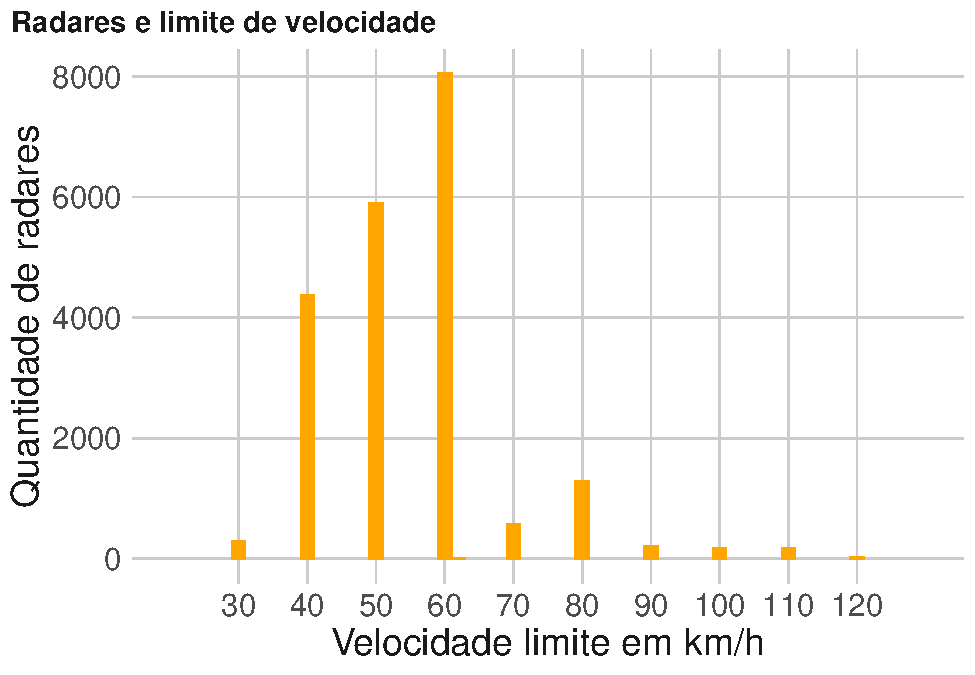
\includegraphics{RelatorioVelocidades_files/figure-latex/unnamed-chunk-20-1.pdf}

\chapter{Correlações}\label{correlauxe7uxf5es}

\section{Bibliotecas}\label{bibliotecas-4}

Foram utilizadas diversas bibliotecas nessa seção, sendo elas:

\begin{Shaded}
\begin{Highlighting}[]
\FunctionTok{library}\NormalTok{(}\StringTok{\textquotesingle{}readxl\textquotesingle{}}\NormalTok{) }\CommentTok{\#ler arquivo xlsx excel}
\FunctionTok{library}\NormalTok{(}\StringTok{\textquotesingle{}tidyverse\textquotesingle{}}\NormalTok{) }\CommentTok{\# plotar gráficos e utilizar o pipe}
\FunctionTok{library}\NormalTok{(}\StringTok{\textquotesingle{}patchwork\textquotesingle{}}\NormalTok{) }\CommentTok{\# plotar gráficos juntos}
\FunctionTok{library}\NormalTok{(}\StringTok{\textquotesingle{}onsvplot\textquotesingle{}}\NormalTok{) }\CommentTok{\# usar o tema de gráfico do onsv}
\FunctionTok{library}\NormalTok{(}\StringTok{\textquotesingle{}corrplot\textquotesingle{}}\NormalTok{) }\CommentTok{\# fazer o correlograma}
\CommentTok{\# devtools::install\_github("pabsantos/roadtrafficdeaths")}
\CommentTok{\# devtools::install\_github("jotasaraiva/fleetbr")}
\FunctionTok{library}\NormalTok{(}\StringTok{\textquotesingle{}roadtrafficdeaths\textquotesingle{}}\NormalTok{) }\CommentTok{\# dados sobre mortalidade no trânsito}
\FunctionTok{library}\NormalTok{(}\StringTok{\textquotesingle{}fleetbr\textquotesingle{}}\NormalTok{) }\CommentTok{\# dados sobre a frota de veículos}
\end{Highlighting}
\end{Shaded}

\section{Importando os dados e manipulando estruturas}\label{importando-os-dados-e-manipulando-estruturas}

Foi importado os dados relativos as infrações e retirado a linha ``BR'', além de renomear a coluna relativo ao indicador de infrações. Com isso foi feito uma união com o \emph{Data Frame} criado no capítulo \hyperref[radar-frota]{2} e trocado onde havia \texttt{NA} por 0.

\begin{Shaded}
\begin{Highlighting}[]
\NormalTok{infrações }\OtherTok{\textless{}{-}} \FunctionTok{read\_xlsx}\NormalTok{(}\StringTok{"/home/silvana/Downloads/INDICADORES\_RADARES\_VELOCIDADE\_UF (indicador velocidade, infrações, mortalidade)).xlsx"}\NormalTok{, }\AttributeTok{sheet =} \DecValTok{7}\NormalTok{)}
\NormalTok{infrações }\OtherTok{\textless{}{-}}\NormalTok{ infrações[}\SpecialCharTok{{-}}\DecValTok{7}\NormalTok{,] }\CommentTok{\#excluindo a linha "BR"}
\NormalTok{infrações }\OtherTok{\textless{}{-}} \FunctionTok{rename}\NormalTok{(infrações, infrações }\OtherTok{=} \StringTok{\textasciigrave{}}\AttributeTok{infrações/10000 veículos}\StringTok{\textasciigrave{}}\NormalTok{)}

\NormalTok{Indicador\_radares }\OtherTok{\textless{}{-}} \FunctionTok{rename}\NormalTok{(Indicador\_radares, }\AttributeTok{UF =}\NormalTok{ SiglaUf) }\CommentTok{\#Esse data frame vem do script "Indicadores radares\_frota.R"}

\NormalTok{rad\_inf }\OtherTok{\textless{}{-}} \FunctionTok{full\_join}\NormalTok{(infrações[,}\FunctionTok{c}\NormalTok{(}\DecValTok{1}\NormalTok{,}\DecValTok{4}\NormalTok{)], Indicador\_radares, }\AttributeTok{by =} \StringTok{"UF"}\NormalTok{)}

\NormalTok{rad\_inf }\OtherTok{\textless{}{-}}\NormalTok{ rad\_inf }\SpecialCharTok{\%\textgreater{}\%} 
  \FunctionTok{mutate\_all}\NormalTok{(replace\_na, }\DecValTok{0}\NormalTok{)}
\end{Highlighting}
\end{Shaded}

\section{Gráficos}\label{gruxe1ficos}

Foi feito então um gráfico geral para avaliar a correlação visual entre os indicadores radar/frota e o indicador de infrações.

\begin{Shaded}
\begin{Highlighting}[]
\FunctionTok{ggplot}\NormalTok{(}\AttributeTok{data =}\NormalTok{ rad\_inf)}\SpecialCharTok{+}
  \FunctionTok{geom\_point}\NormalTok{(}\AttributeTok{mapping =} \FunctionTok{aes}\NormalTok{(}\AttributeTok{x=}\NormalTok{ infrações , }\AttributeTok{y =}\NormalTok{ i1))}\SpecialCharTok{+}
  \FunctionTok{geom\_smooth}\NormalTok{(}\AttributeTok{mapping =} \FunctionTok{aes}\NormalTok{(}\AttributeTok{x=}\NormalTok{ infrações , }\AttributeTok{y =}\NormalTok{ i1), }\AttributeTok{se =} \ConstantTok{FALSE}\NormalTok{)}\SpecialCharTok{+}\FunctionTok{theme\_onsv}\NormalTok{()}\SpecialCharTok{+}
  \FunctionTok{ggplot}\NormalTok{(}\AttributeTok{data =}\NormalTok{ rad\_inf)}\SpecialCharTok{+}
  \FunctionTok{geom\_point}\NormalTok{(}\AttributeTok{mapping =} \FunctionTok{aes}\NormalTok{(}\AttributeTok{x=}\NormalTok{ infrações , }\AttributeTok{y =}\NormalTok{ i2))}\SpecialCharTok{+}
  \FunctionTok{geom\_smooth}\NormalTok{(}\AttributeTok{mapping =} \FunctionTok{aes}\NormalTok{(}\AttributeTok{x=}\NormalTok{ infrações, }\AttributeTok{y =}\NormalTok{ i2), }\AttributeTok{se =} \ConstantTok{FALSE}\NormalTok{)}\SpecialCharTok{+}\FunctionTok{theme\_onsv}\NormalTok{()}\SpecialCharTok{+}
  \FunctionTok{ggplot}\NormalTok{(}\AttributeTok{data =}\NormalTok{ rad\_inf)}\SpecialCharTok{+}
  \FunctionTok{geom\_point}\NormalTok{(}\AttributeTok{mapping =} \FunctionTok{aes}\NormalTok{(}\AttributeTok{x=}\NormalTok{ infrações, }\AttributeTok{y =}\NormalTok{ i3))}\SpecialCharTok{+}
  \FunctionTok{geom\_smooth}\NormalTok{(}\AttributeTok{mapping =} \FunctionTok{aes}\NormalTok{(}\AttributeTok{x=}\NormalTok{ infrações, }\AttributeTok{y =}\NormalTok{ i3), }\AttributeTok{se =} \ConstantTok{FALSE}\NormalTok{)}\SpecialCharTok{+}\FunctionTok{theme\_onsv}\NormalTok{()}\SpecialCharTok{+}
  \FunctionTok{ggplot}\NormalTok{(}\AttributeTok{data =}\NormalTok{ rad\_inf)}\SpecialCharTok{+}
  \FunctionTok{geom\_point}\NormalTok{(}\AttributeTok{mapping =} \FunctionTok{aes}\NormalTok{(}\AttributeTok{x=}\NormalTok{ infrações , }\AttributeTok{y =}\NormalTok{ i4))}\SpecialCharTok{+}
  \FunctionTok{geom\_smooth}\NormalTok{(}\AttributeTok{mapping =} \FunctionTok{aes}\NormalTok{(}\AttributeTok{x=}\NormalTok{ infrações, }\AttributeTok{y =}\NormalTok{ i4), }\AttributeTok{se =} \ConstantTok{FALSE}\NormalTok{)}\SpecialCharTok{+}\FunctionTok{theme\_onsv}\NormalTok{()}\SpecialCharTok{+}
  \FunctionTok{ggplot}\NormalTok{(}\AttributeTok{data =}\NormalTok{ rad\_inf)}\SpecialCharTok{+}
  \FunctionTok{geom\_point}\NormalTok{(}\AttributeTok{mapping =} \FunctionTok{aes}\NormalTok{(}\AttributeTok{x=}\NormalTok{ infrações , }\AttributeTok{y =}\NormalTok{ i5))}\SpecialCharTok{+}
  \FunctionTok{geom\_smooth}\NormalTok{(}\AttributeTok{mapping =} \FunctionTok{aes}\NormalTok{(}\AttributeTok{x=}\NormalTok{ infrações , }\AttributeTok{y =}\NormalTok{ i5), }\AttributeTok{se =} \ConstantTok{FALSE}\NormalTok{)}\SpecialCharTok{+}\FunctionTok{theme\_onsv}\NormalTok{()}\SpecialCharTok{+}
  \FunctionTok{ggplot}\NormalTok{(}\AttributeTok{data =}\NormalTok{ rad\_inf)}\SpecialCharTok{+}
  \FunctionTok{geom\_point}\NormalTok{(}\AttributeTok{mapping =} \FunctionTok{aes}\NormalTok{(}\AttributeTok{x=}\NormalTok{ infrações, }\AttributeTok{y =}\NormalTok{ i6))}\SpecialCharTok{+}
  \FunctionTok{geom\_smooth}\NormalTok{(}\AttributeTok{mapping =} \FunctionTok{aes}\NormalTok{(}\AttributeTok{x=}\NormalTok{ infrações, }\AttributeTok{y =}\NormalTok{ i6), }\AttributeTok{se =} \ConstantTok{FALSE}\NormalTok{)}\SpecialCharTok{+}\FunctionTok{theme\_onsv}\NormalTok{()}\SpecialCharTok{+}
  \FunctionTok{ggplot}\NormalTok{(}\AttributeTok{data =}\NormalTok{ rad\_inf)}\SpecialCharTok{+}
  \FunctionTok{geom\_point}\NormalTok{(}\AttributeTok{mapping =} \FunctionTok{aes}\NormalTok{(}\AttributeTok{x=}\NormalTok{ infrações , }\AttributeTok{y =}\NormalTok{ i7))}\SpecialCharTok{+}
  \FunctionTok{geom\_smooth}\NormalTok{(}\AttributeTok{mapping =} \FunctionTok{aes}\NormalTok{(}\AttributeTok{x=}\NormalTok{ infrações , }\AttributeTok{y =}\NormalTok{ i7), }\AttributeTok{se =} \ConstantTok{FALSE}\NormalTok{)}\SpecialCharTok{+}\FunctionTok{theme\_onsv}\NormalTok{()}\SpecialCharTok{+}
  \FunctionTok{ggplot}\NormalTok{(}\AttributeTok{data =}\NormalTok{ rad\_inf)}\SpecialCharTok{+}
  \FunctionTok{geom\_point}\NormalTok{(}\AttributeTok{mapping =} \FunctionTok{aes}\NormalTok{(}\AttributeTok{x=}\NormalTok{ infrações, }\AttributeTok{y =}\NormalTok{ i8))}\SpecialCharTok{+}
  \FunctionTok{geom\_smooth}\NormalTok{(}\AttributeTok{mapping =} \FunctionTok{aes}\NormalTok{(}\AttributeTok{x=}\NormalTok{ infrações, }\AttributeTok{y =}\NormalTok{ i8), }\AttributeTok{se =} \ConstantTok{FALSE}\NormalTok{)}\SpecialCharTok{+}\FunctionTok{theme\_onsv}\NormalTok{()}\SpecialCharTok{+}
  \FunctionTok{ggplot}\NormalTok{(}\AttributeTok{data =}\NormalTok{ rad\_inf)}\SpecialCharTok{+}
  \FunctionTok{geom\_point}\NormalTok{(}\AttributeTok{mapping =} \FunctionTok{aes}\NormalTok{(}\AttributeTok{x=}\NormalTok{ infrações , }\AttributeTok{y =}\NormalTok{ i9))}\SpecialCharTok{+}
  \FunctionTok{geom\_smooth}\NormalTok{(}\AttributeTok{mapping =} \FunctionTok{aes}\NormalTok{(}\AttributeTok{x=}\NormalTok{ infrações, }\AttributeTok{y =}\NormalTok{ i9), }\AttributeTok{se =} \ConstantTok{FALSE}\NormalTok{)}\SpecialCharTok{+}\FunctionTok{theme\_onsv}\NormalTok{()}
\end{Highlighting}
\end{Shaded}

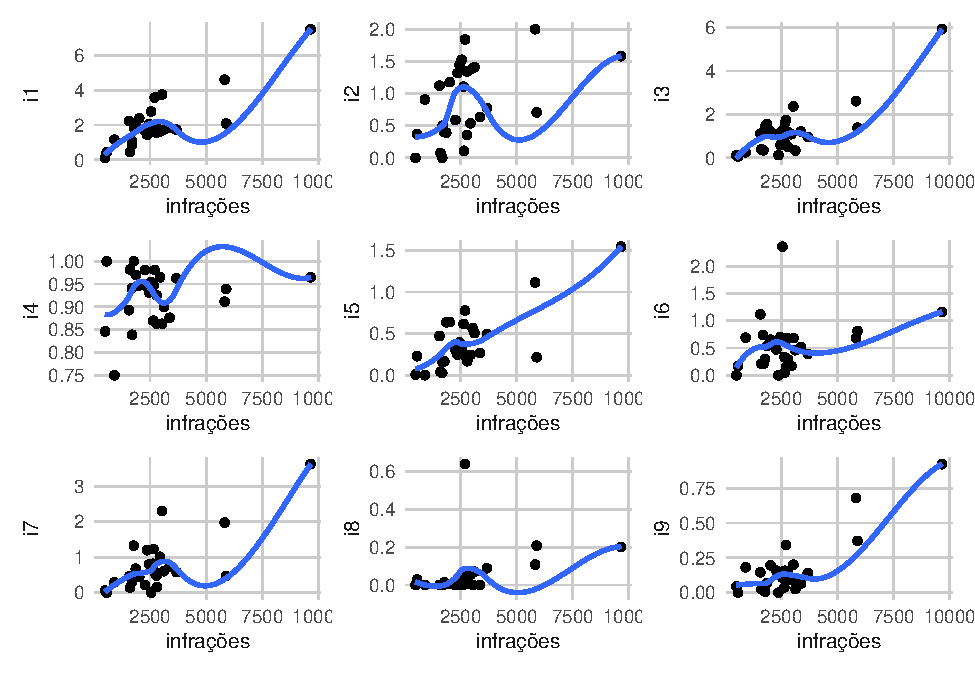
\includegraphics{RelatorioVelocidades_files/figure-latex/unnamed-chunk-23-1.pdf}
Mas por fim foi adicionado no relatório apenas o gráfico de I\textsubscript{1} \emph{vs} infrações.

\begin{Shaded}
\begin{Highlighting}[]
\FunctionTok{ggplot}\NormalTok{(}\AttributeTok{data =}\NormalTok{ rad\_inf)}\SpecialCharTok{+}
  \FunctionTok{geom\_point}\NormalTok{(}\AttributeTok{mapping =} \FunctionTok{aes}\NormalTok{(}\AttributeTok{x=}\NormalTok{ infrações , }\AttributeTok{y =}\NormalTok{ i1))}\SpecialCharTok{+}
  \FunctionTok{geom\_smooth}\NormalTok{(}\AttributeTok{mapping =} \FunctionTok{aes}\NormalTok{(}\AttributeTok{x=}\NormalTok{ infrações , }\AttributeTok{y =}\NormalTok{ i1), }\AttributeTok{se =} \ConstantTok{FALSE}\NormalTok{, }\AttributeTok{method =} \StringTok{"lm"}\NormalTok{)}\SpecialCharTok{+}
  \FunctionTok{theme\_onsv}\NormalTok{()}\SpecialCharTok{+}
  \FunctionTok{labs}\NormalTok{(}\AttributeTok{x =} \StringTok{"Quantidade de infrações a cada 10 mil veículos"}\NormalTok{, }\AttributeTok{y=}\StringTok{"I1 {-} Quantidade geral de radares a cada 10 mil veículos"}\NormalTok{)}\SpecialCharTok{+}
  \FunctionTok{theme}\NormalTok{(}\AttributeTok{axis.title.x =} \FunctionTok{element\_text}\NormalTok{(}\AttributeTok{size =}\DecValTok{18}\NormalTok{),}\AttributeTok{axis.title.y =} \FunctionTok{element\_text}\NormalTok{(}\AttributeTok{size =}\DecValTok{10}\NormalTok{))}
\end{Highlighting}
\end{Shaded}

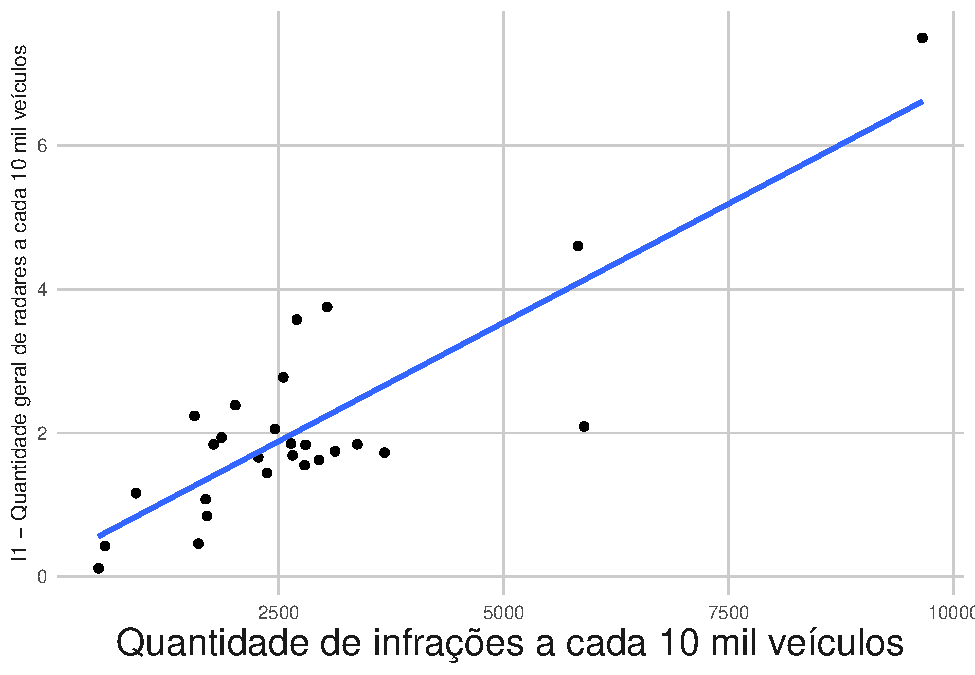
\includegraphics{RelatorioVelocidades_files/figure-latex/unnamed-chunk-24-1.pdf}
Nesse arquivo \emph{bookdown} eu tive que diminuir o tamanho da legenda do eixo ``y'' para 10 pois não estava ``cabendo'' no gráfico, mas no relatório foi utilizado a fonte 18 para o eixo ``y'' (o mesmo tamanho da fonte do eixo ``x'')

\section{Correlograma entre indicadores radar/frota e indicador infrações}\label{correlograma-entre-indicadores-radarfrota-e-indicador-infrauxe7uxf5es}

Foi feito um \texttt{cor.test()} em todos os casos para verificar se são estatísticamente correlacionados:

\begin{Shaded}
\begin{Highlighting}[]
\FunctionTok{cor.test}\NormalTok{(rad\_inf}\SpecialCharTok{$}\NormalTok{infrações, rad\_inf}\SpecialCharTok{$}\NormalTok{i1, }\AttributeTok{method =} \StringTok{\textquotesingle{}spearman\textquotesingle{}}\NormalTok{)}
\FunctionTok{cor.test}\NormalTok{(rad\_inf}\SpecialCharTok{$}\NormalTok{infrações, rad\_inf}\SpecialCharTok{$}\NormalTok{i2, }\AttributeTok{method =} \StringTok{\textquotesingle{}spearman\textquotesingle{}}\NormalTok{)}
\FunctionTok{cor.test}\NormalTok{(rad\_inf}\SpecialCharTok{$}\NormalTok{infrações, rad\_inf}\SpecialCharTok{$}\NormalTok{i3, }\AttributeTok{method =} \StringTok{\textquotesingle{}spearman\textquotesingle{}}\NormalTok{)}
\FunctionTok{cor.test}\NormalTok{(rad\_inf}\SpecialCharTok{$}\NormalTok{infrações, rad\_inf}\SpecialCharTok{$}\NormalTok{i4, }\AttributeTok{method =} \StringTok{\textquotesingle{}spearman\textquotesingle{}}\NormalTok{)}
\FunctionTok{cor.test}\NormalTok{(rad\_inf}\SpecialCharTok{$}\NormalTok{infrações, rad\_inf}\SpecialCharTok{$}\NormalTok{i5, }\AttributeTok{method =} \StringTok{\textquotesingle{}spearman\textquotesingle{}}\NormalTok{)}
\FunctionTok{cor.test}\NormalTok{(rad\_inf}\SpecialCharTok{$}\NormalTok{infrações, rad\_inf}\SpecialCharTok{$}\NormalTok{i6, }\AttributeTok{method =} \StringTok{\textquotesingle{}spearman\textquotesingle{}}\NormalTok{)}
\FunctionTok{cor.test}\NormalTok{(rad\_inf}\SpecialCharTok{$}\NormalTok{infrações, rad\_inf}\SpecialCharTok{$}\NormalTok{i7, }\AttributeTok{method =} \StringTok{\textquotesingle{}spearman\textquotesingle{}}\NormalTok{)}
\FunctionTok{cor.test}\NormalTok{(rad\_inf}\SpecialCharTok{$}\NormalTok{infrações, rad\_inf}\SpecialCharTok{$}\NormalTok{i8, }\AttributeTok{method =} \StringTok{\textquotesingle{}spearman\textquotesingle{}}\NormalTok{)}
\FunctionTok{cor.test}\NormalTok{(rad\_inf}\SpecialCharTok{$}\NormalTok{infrações, rad\_inf}\SpecialCharTok{$}\NormalTok{i9, }\AttributeTok{method =} \StringTok{\textquotesingle{}spearman\textquotesingle{}}\NormalTok{)}
\end{Highlighting}
\end{Shaded}

Com isso ficou nítido que o I\textsubscript{4} não possui correlação algumas com as infrações e o I\textsubscript{6}também poderia ser excluido se considerassemos um p-valor\textless0.05.\\
Após esse teste, foi feito o gráfico de correlação geral:

\begin{Shaded}
\begin{Highlighting}[]
\NormalTok{graf\_corr }\OtherTok{\textless{}{-}} \FunctionTok{cor}\NormalTok{(rad\_inf[,}\FunctionTok{c}\NormalTok{(}\SpecialCharTok{{-}}\DecValTok{1}\NormalTok{,}\SpecialCharTok{{-}}\DecValTok{6}\NormalTok{)], }\AttributeTok{method =} \StringTok{"spearman"}\NormalTok{)}

\FunctionTok{corrplot}\NormalTok{(graf\_corr, }\AttributeTok{type =} \StringTok{"lower"}\NormalTok{, }\AttributeTok{method =} \StringTok{"number"}\NormalTok{) }
\end{Highlighting}
\end{Shaded}

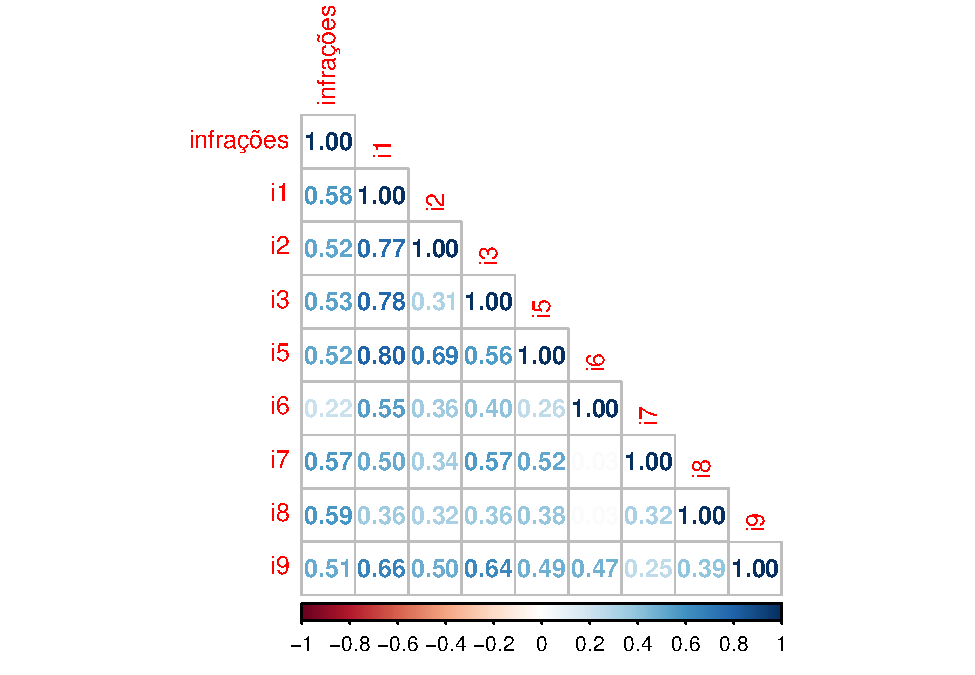
\includegraphics{RelatorioVelocidades_files/figure-latex/unnamed-chunk-26-1.pdf}
\#\# Correlação entre infrações e mortalidade\\
Para esse correlação foi feito um ajuste na base de dados do DataSus e teve de ser criado um \texttt{tibble}(um \emph{Data Frame} evoluído) sobre as regiões das unidades da federação, classificando cada unidade da federação na sua respectiva região. Fazendo então a união de três bases, a base de mortalidade, a base de infrações e a base das regiões.

\begin{Shaded}
\begin{Highlighting}[]
\NormalTok{rtdeaths\_2022}\OtherTok{\textless{}{-}} \FunctionTok{filter}\NormalTok{(rtdeaths,rtdeaths}\SpecialCharTok{$}\NormalTok{ano\_ocorrencia }\SpecialCharTok{==} \DecValTok{2022}\NormalTok{)}
\NormalTok{rtdeaths\_2022 }\OtherTok{\textless{}{-}}\NormalTok{ rtdeaths\_2022 }\SpecialCharTok{\%\textgreater{}\%}
  \FunctionTok{group\_by}\NormalTok{(rtdeaths\_2022}\SpecialCharTok{$}\NormalTok{nome\_uf\_ocor) }\SpecialCharTok{\%\textgreater{}\%}
  \FunctionTok{summarise}\NormalTok{(}
    \AttributeTok{quantidade =} \FunctionTok{n}\NormalTok{()}
\NormalTok{  )}
\NormalTok{rtdeaths\_2022 }\OtherTok{\textless{}{-}}\NormalTok{ rtdeaths\_2022[}\SpecialCharTok{{-}}\DecValTok{28}\NormalTok{,]}
\NormalTok{rtdeaths\_2022 }\OtherTok{\textless{}{-}} \FunctionTok{mutate}\NormalTok{(rtdeaths\_2022,  }\AttributeTok{UF =} \FunctionTok{c}\NormalTok{(}\StringTok{"AC"}\NormalTok{, }\StringTok{"AL"}\NormalTok{, }\StringTok{"AP"}\NormalTok{, }\StringTok{"AM"}\NormalTok{, }\StringTok{"BA"}\NormalTok{, }\StringTok{"CE"}\NormalTok{, }\StringTok{"DF"}\NormalTok{, }\StringTok{"ES"}\NormalTok{, }\StringTok{"GO"}\NormalTok{, }\StringTok{"MA"}\NormalTok{, }\StringTok{"MT"}\NormalTok{, }
                                               \StringTok{"MS"}\NormalTok{, }\StringTok{"MG"}\NormalTok{, }\StringTok{"PR"}\NormalTok{, }\StringTok{"PB"}\NormalTok{, }
                                               \StringTok{"PA"}\NormalTok{, }\StringTok{"PE"}\NormalTok{, }\StringTok{"PI"}\NormalTok{, }\StringTok{"RN"}\NormalTok{, }\StringTok{"RS"}\NormalTok{, }\StringTok{"RJ"}\NormalTok{, }\StringTok{"RO"}\NormalTok{, }\StringTok{"RR"}\NormalTok{, }\StringTok{"SC"}\NormalTok{, }\StringTok{"SE"}\NormalTok{, }\StringTok{"SP"}\NormalTok{, }\StringTok{"TO"}\NormalTok{))}
\NormalTok{rtdeaths\_2022 }\OtherTok{\textless{}{-}} \FunctionTok{rename}\NormalTok{(rtdeaths\_2022, }\AttributeTok{Estado =} \StringTok{\textasciigrave{}}\AttributeTok{rtdeaths\_2022$nome\_uf\_ocor}\StringTok{\textasciigrave{}}\NormalTok{)}

\NormalTok{fleet\_2022 }\OtherTok{\textless{}{-}} \FunctionTok{filter}\NormalTok{(fleetbr, mes }\SpecialCharTok{==} \DecValTok{12}\NormalTok{, ano }\SpecialCharTok{==} \DecValTok{2022}\NormalTok{, modal }\SpecialCharTok{==} \StringTok{"TOTAL"}\NormalTok{)}

\NormalTok{rtdeaths\_fleet }\OtherTok{\textless{}{-}} \FunctionTok{inner\_join}\NormalTok{(rtdeaths\_2022, fleet\_2022, }\AttributeTok{by =} \FunctionTok{c}\NormalTok{(}\StringTok{"UF"} \OtherTok{=} \StringTok{"uf"}\NormalTok{))}
\NormalTok{rtdeaths\_fleet }\OtherTok{\textless{}{-}} \FunctionTok{mutate}\NormalTok{(rtdeaths\_fleet, }\AttributeTok{A\_cada\_10\_mil =}\NormalTok{ (quantidade}\SpecialCharTok{*}\DecValTok{10}\SpecialCharTok{\^{}}\DecValTok{4}\NormalTok{)}\SpecialCharTok{/}\NormalTok{frota)}

\NormalTok{rad\_inf2 }\OtherTok{\textless{}{-}} \FunctionTok{subset}\NormalTok{(rad\_inf, }\AttributeTok{select =}\NormalTok{ infrações)}
\FunctionTok{cor.test}\NormalTok{(rad\_inf2}\SpecialCharTok{$}\NormalTok{infrações,rtdeaths\_fleet}\SpecialCharTok{$}\NormalTok{A\_cada\_10\_mil, }\AttributeTok{method =} \StringTok{"spearman"}\NormalTok{)}
\end{Highlighting}
\end{Shaded}

\begin{verbatim}
## 
##  Spearman's rank correlation rho
## 
## data:  rad_inf2$infrações and rtdeaths_fleet$A_cada_10_mil
## S = 3108, p-value = 0.7992
## alternative hypothesis: true rho is not equal to 0
## sample estimates:
##        rho 
## 0.05128205
\end{verbatim}

\begin{Shaded}
\begin{Highlighting}[]
\FunctionTok{cor.test}\NormalTok{(rad\_inf}\SpecialCharTok{$}\NormalTok{i1,rtdeaths\_fleet}\SpecialCharTok{$}\NormalTok{A\_cada\_10\_mil, }\AttributeTok{method =} \StringTok{"spearman"}\NormalTok{)}
\end{Highlighting}
\end{Shaded}

\begin{verbatim}
## 
##  Spearman's rank correlation rho
## 
## data:  rad_inf$i1 and rtdeaths_fleet$A_cada_10_mil
## S = 3796, p-value = 0.4274
## alternative hypothesis: true rho is not equal to 0
## sample estimates:
##        rho 
## -0.1587302
\end{verbatim}

\begin{Shaded}
\begin{Highlighting}[]
\NormalTok{mort\_ind }\OtherTok{\textless{}{-}}\NormalTok{ rtdeaths\_fleet }\SpecialCharTok{\%\textgreater{}\%} 
  \FunctionTok{inner\_join}\NormalTok{(rad\_inf, }\AttributeTok{by =} \StringTok{"UF"}\NormalTok{)}

\NormalTok{regioes }\OtherTok{\textless{}{-}} \FunctionTok{tibble}\NormalTok{(}\AttributeTok{UF =} \FunctionTok{c}\NormalTok{(}\StringTok{"RS"}\NormalTok{,}\StringTok{"SC"}\NormalTok{,}\StringTok{"PR"}\NormalTok{,}\StringTok{"SP"}\NormalTok{,}\StringTok{"MG"}\NormalTok{,}\StringTok{"RJ"}\NormalTok{,}\StringTok{"ES"}\NormalTok{,}\StringTok{"MS"}\NormalTok{,}\StringTok{"MT"}\NormalTok{,}\StringTok{"GO"}\NormalTok{,}\StringTok{"DF"}\NormalTok{,}\StringTok{"BA"}\NormalTok{,}\StringTok{"SE"}\NormalTok{,}\StringTok{"AL"}\NormalTok{,}\StringTok{"PE"}\NormalTok{,}\StringTok{"PB"}\NormalTok{,}\StringTok{"RN"}\NormalTok{,}\StringTok{"CE"}\NormalTok{,}\StringTok{"PI"}\NormalTok{,}\StringTok{"MA"}\NormalTok{,}
                            \StringTok{"TO"}\NormalTok{,}\StringTok{"PA"}\NormalTok{,}\StringTok{"AP"}\NormalTok{,}\StringTok{"RR"}\NormalTok{,}\StringTok{"RO"}\NormalTok{,}\StringTok{"AM"}\NormalTok{,}\StringTok{"AC"}\NormalTok{),}
                  \AttributeTok{Regiao =} \FunctionTok{c}\NormalTok{(}\StringTok{"Sul"}\NormalTok{,}\StringTok{"Sul"}\NormalTok{,}\StringTok{"Sul"}\NormalTok{,}\StringTok{"Sudeste"}\NormalTok{,}\StringTok{"Sudeste"}\NormalTok{,}\StringTok{"Sudeste"}\NormalTok{,}\StringTok{"Sudeste"}\NormalTok{,}\StringTok{"Centro Oeste"}\NormalTok{,}\StringTok{"Centro Oeste"}\NormalTok{,}
                             \StringTok{"Centro Oeste"}\NormalTok{,}\StringTok{"Centro Oeste"}\NormalTok{,}\StringTok{"Nordeste"}\NormalTok{,}\StringTok{"Nordeste"}\NormalTok{,}\StringTok{"Nordeste"}\NormalTok{,}\StringTok{"Nordeste"}\NormalTok{,}\StringTok{"Nordeste"}\NormalTok{,}\StringTok{"Nordeste"}\NormalTok{,}
                             \StringTok{"Nordeste"}\NormalTok{,}\StringTok{"Nordeste"}\NormalTok{,}\StringTok{"Nordeste"}\NormalTok{,}\StringTok{"Norte"}\NormalTok{,}\StringTok{"Norte"}\NormalTok{,}\StringTok{"Norte"}\NormalTok{,}\StringTok{"Norte"}\NormalTok{,}\StringTok{"Norte"}\NormalTok{,}\StringTok{"Norte"}\NormalTok{,}\StringTok{"Norte"}\NormalTok{))}
\NormalTok{mort\_ind }\OtherTok{\textless{}{-}}\NormalTok{ mort\_ind }\SpecialCharTok{\%\textgreater{}\%}
  \FunctionTok{inner\_join}\NormalTok{(regioes, }\AttributeTok{by =} \StringTok{"UF"}\NormalTok{)}
\end{Highlighting}
\end{Shaded}

Note também que foi feito um teste de correlação, e ele já indicou que não há tal correlação, mas mesmo assim podemos tirar \emph{insights} visuais do gráfico feito abaixo:

\begin{Shaded}
\begin{Highlighting}[]
\FunctionTok{ggplot}\NormalTok{(}\AttributeTok{data =}\NormalTok{ mort\_ind)}\SpecialCharTok{+}
  \FunctionTok{geom\_point}\NormalTok{(}\AttributeTok{mapping =} \FunctionTok{aes}\NormalTok{(}\AttributeTok{x =}\NormalTok{ i1, }\AttributeTok{y =}\NormalTok{ A\_cada\_10\_mil, }\AttributeTok{color =}\NormalTok{ Regiao))}\SpecialCharTok{+}
  \FunctionTok{geom\_label}\NormalTok{(}\FunctionTok{aes}\NormalTok{(}\AttributeTok{x =}\NormalTok{ i1, }\AttributeTok{y =}\NormalTok{ A\_cada\_10\_mil, }\AttributeTok{label =}\NormalTok{ UF), }\AttributeTok{size =} \FloatTok{3.5}\NormalTok{, }\AttributeTok{hjust =} \SpecialCharTok{{-}}\FloatTok{0.3}\NormalTok{)}\SpecialCharTok{+}
  \FunctionTok{theme\_onsv}\NormalTok{()}\SpecialCharTok{+}
  \FunctionTok{labs}\NormalTok{(}\AttributeTok{x =} \StringTok{"I1 {-} Quantidade de radares a cada 10 mil veículos"}\NormalTok{, }\AttributeTok{y =} \StringTok{"Mortes a cada 10 mil veículos"}\NormalTok{)}\SpecialCharTok{+}
  \FunctionTok{theme}\NormalTok{(}\AttributeTok{axis.title.x =} \FunctionTok{element\_text}\NormalTok{(}\AttributeTok{size =}\DecValTok{18}\NormalTok{),}
        \AttributeTok{axis.title.y =} \FunctionTok{element\_text}\NormalTok{(}\AttributeTok{size =}\DecValTok{18}\NormalTok{), }
        \AttributeTok{legend.text =} \FunctionTok{element\_text}\NormalTok{(}\AttributeTok{size =}\DecValTok{12}\NormalTok{))}
\end{Highlighting}
\end{Shaded}

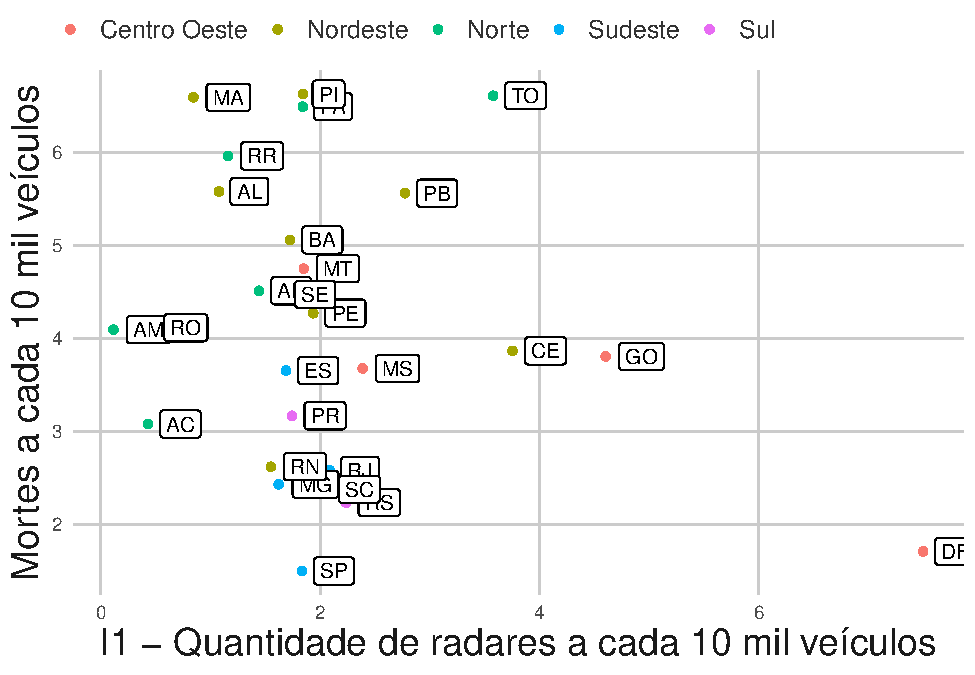
\includegraphics{RelatorioVelocidades_files/figure-latex/unnamed-chunk-28-1.pdf}

  \bibliography{book.bib,packages.bib}

\end{document}
